\section{Comparison of Mutation and Crossover Operators}
\label{exp_crossovers}

In this chapter, we will compare the effectiveness of different crossover types in combination with different mutation operators inside each of the group of crossover operators: path representation (in Section \ref{subsec:experiments_path}) and adjacency representation crossovers (in Section \ref{subsec:experiments_adj}). Moreover, ordinal representation with OPX is discussed in Section \ref{subsec:experiments_ordinal}. The crossover types which showed the best results inside each group combined with the most effective mutation operator will be considered again in the next phase.\par

 According to the results from Section \ref{subsec:parameters_results}, we fix the mutation rate at 3$\%$ and the population size factor as 3 for the following experiments. Like in the previous section, we will use the same evaluation metrics and the same type of selection, namely tournament selection, where the number of participants in the tournament is drawn randomly from the interval $[2, 10]$. The experiments will also be made for each group of instances separately, as we assume that the size of the TSP instances can influence the results.\par 

Please note that due to the shortage of computational time, we will conduct these experiments without using heuristics in the population, that is, the population is initialized with random permutations.\par  


\subsection{Path Representation Crossovers}
\label{subsec:experiments_path}

\subsubsection{Methods}

In this part of our experiments, we will compare the effectiveness of path representation crossover operators with each other, namely modified crossover (MX), order-based (OBX), order crossover (OX), linear order crossover (LOX), position-based crossover (PBX), partially-mapped crossover (PMX), and cycle crossover (CX) (see Section \ref{subsec:path_crossovers}). In addition, we combine these 7 crossover types with 6 different mutation types, namely swap, shift, scramble, inversion, insertion, and displacement (see Section \ref{sec:mutation}).  As a result, we get 42 configurations in total.  \par 


\subsubsection{Results and Discussion}

\begin{figure}[t] \centering
	\centering
	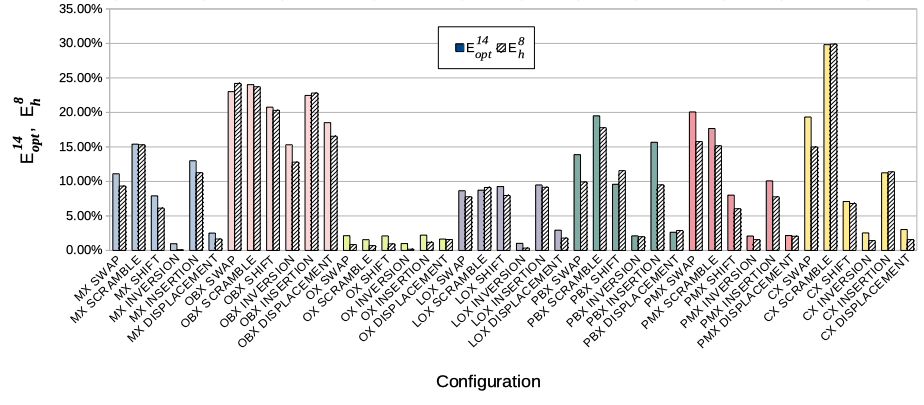
\includegraphics[width=1\textwidth]{9_1_path_less_100}
	\caption{$E_{opt}^{14}$, $E_{h}^{8}$ for instances with less than 100 cities for path representation crossovers.}
	\label{fig:9_1_path_less_100}
\end{figure}

\begin{table}[t] \centering
	\centering
	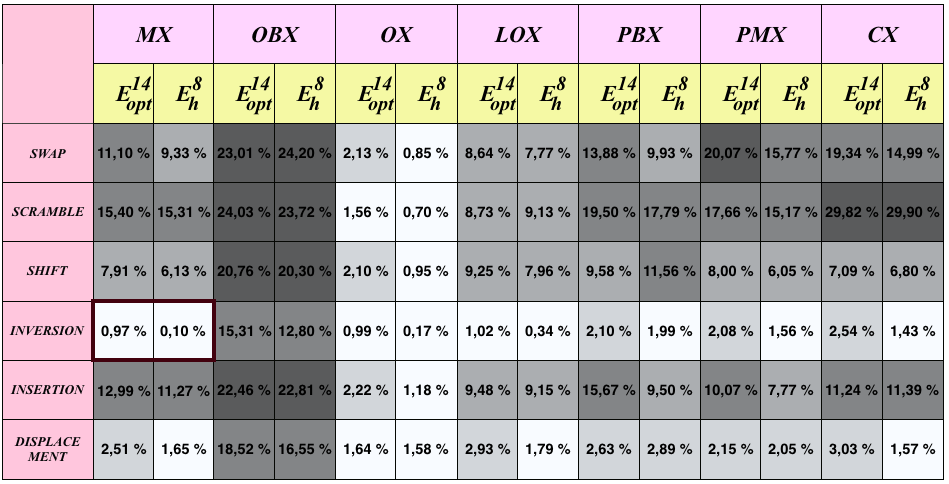
\includegraphics[width=1\textwidth]{tab_9_1_path_less_100}
	\caption{Results for 22 instances with less than 100 cities for 7 path representation crossovers and 6 mutation operators}
	\label{Tab:tab_9_1_path_less_100}
\end{table}

In the group of instances with less than 100 cities the OX showed good results in combination with all mutation types (see Figure \ref{fig:9_1_path_less_100}). One reason for this may be the fact that we used the general parameters which were optimized for this crossover type. However, its performance is much better than the one of other crossover types, and its effectiveness is pointed out in the literature as well (\cite{potvin1996genetic}).\par

The OBX performed worst independent from the type of mutation used with a significant difference from the other crossover types. As it was described in Section \ref{subsubsec:order_based}, if the OBX receives a very small subset of cities to work with, the offspring will be very similar to the second parent chromosome. Perhaps, in our experiments the OBX worked on average on too small subsets, and as we used random permutations to build the initial population in these experiments, the second parent was more probable to encode a relatively bad tour. Thus, the OBX may have often resulted in a weak offspring. \par

Concerning the mutation operators (see Table \ref{Tab:tab_9_1_path_less_100}), the scramble mutation can be considered as less effective in general while the inversion and displacement mutation operators have shown good results. This can be caused by the scramble mutation making too many random permutations and thus destroying many edges while the inversion and displacement mutation preserve more edges from the parents (see Section \ref{sec:mutation}).\par

If we take a look at the concrete combinations, the best results were shown by the MX, the OX, and the LOX with inversion, where the MX with inversion mutation is considered as the winner configuration.\par 

In the group of instances with 200 to 500 cities, the OX has shown good results in combination with all mutation types as well (see Figure \ref{fig:9_1_path_200_to_500}). The OBX has shown worst results in combinations with all mutation operators.\par

\begin{figure}[htp] \centering
	\centering
	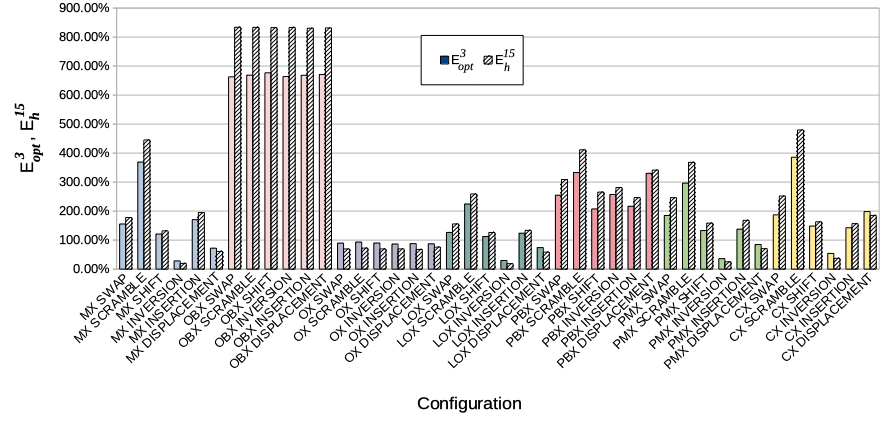
\includegraphics[width=1\textwidth]{9_1_path_200_to_500}
	\caption{$E_{opt}^{14}$, $E_{h}^{8}$ for instances with 200 to 500 cities for path representation crossovers.}
	\label{fig:9_1_path_200_to_500}
\end{figure}

\begin{table}[htp] \centering
	\centering
	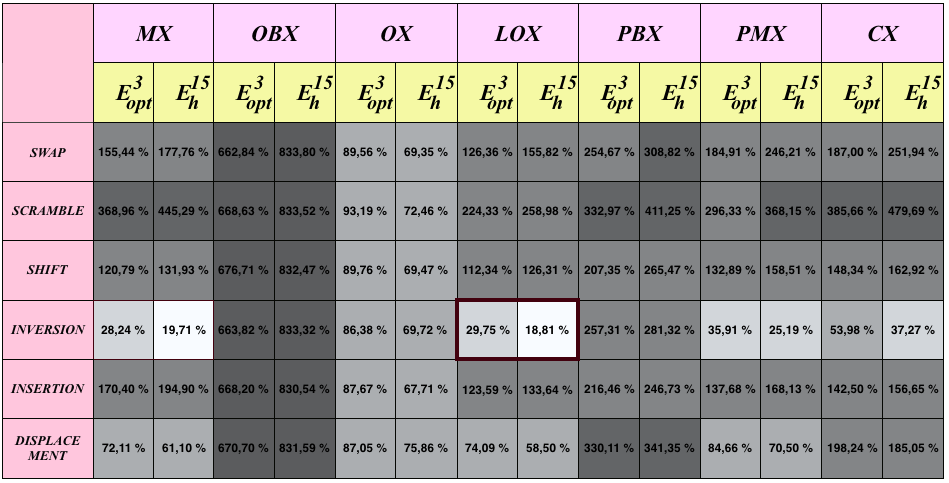
\includegraphics[width=1\textwidth]{tab_9_1_path_200_to_500}
	\caption{Results for 18 instances with 200 to 500 cities for 7 path representation crossovers and 6 mutation operators}
	\label{Tab:tab_9_1_path_200_to_500}
\end{table}

Among the separate configurations, the MX, the LOX, and the PMX all combined with the inversion mutation performed at best. The LOX with inversion mutation is considered as the winner configuration, as it is slightly better than the MX concerning $E^{15}_{h}$ category, where 15 instances were used in comparison with only 3 instances for $E^{3}_{opt}$. \par 

If we take a look at the results grouping them according to mutation types, the inversion and displacement mutation operators seem to be generally better than the other types while the scramble mutation has showed relatively bad results (see Table \ref{Tab:tab_9_1_path_200_to_500}). \par 

In Section \ref{subsec:path_crossovers}, we have considered two groups of crossover operators, namely crossover operators preserving absolute positions (PMX, CX) and crossover operators preserving relative order (MX, OBX, OX, LOX, PBX) to analyze whether one of the groups is generally better than the other. According to \citeauthor{potvin1996genetic} \cite{potvin1996genetic} the crossover operators which preserve relative order perform much better than the crossover operators which preserve absolute order. In his review he referred to the results made by \citeauthor{oliver1987study} \cite{oliver1987study} and the results made by \citeauthor{starkweather1991comparison} \cite{starkweather1991comparison}. \citeauthor{oliver1987study} compared only three operators, namely the OX, the PMX, and CX. Our results confirmed their studies: the OX has performed much better than the PMX and the CX. Of course, the OX has got an advantage because the hyperparameters were tuned for it, but still the difference in performance which it showed is considerable. \par
 
 If we take a look at the experiments conducted by \citeauthor{starkweather1991comparison} \cite{starkweather1991comparison}, they considered 5 crossover operators of the path representation type, namely the OX, the OBX, and the PBX which preserve relative order, and the PMX and the CX which preserve the absolute positions. They used only one very small TSP instance with 30 cities fixing population size at 500 with 50000 generations and no mutation was used with one exception: Some unspecified mutation was used in the CX if the offspring and one of the parents were identical. In their study, the group of crossover operators preserving the relative order has shown much better results than the group with the ones preserving the absolute positions. The OX has performed at best with a strong dominance. Our results were averaged over 40 instances, always used mutation and considered two more representatives of the group of crossovers preserving the relative order, namely MX and LOX. Our results confirmed the dominance of the OX. In difference to our experiments, the OBX has however shown not the worst results here. The PMX and the CX performed worst. However, these two last operators used for some unknown reason larger population of 1400 and 1500 chromosomes, correspondingly, while the other operators worked with 1000 chromosomes.  If we do not consider the OBX which performed worst in our experiments, in general the operators of the group preserving the relative order performed better than the operators of the first group. It is interesting to mention that the MX was not used in the mentioned studies, although it has shown one of the best results in our experiments.\par 

It is obvious that for larger instances with 200 to 500 cities the genetic algorithm performed approximately 10 times worse than for smaller instances with less than 100 cities. This could be perhaps explained by the fact that the genetic algorithm made less iterations for larger instances; therefore, it had no enough time to discover good solutions. \par 

Finally, as it was mentioned in Section \ref{subsec:path_crossovers}, the LOX works similar to the OX, and the PBX is similar to the LOX. It is interesting that in these experiments, the OX has performed better on average than the LOX, and the LOX has shown better results than the PBX. However, this tendency could be influenced by the choice of the used parameters which were tuned specifically for the OX. Nevertheless, due to its good performance here, we will consider the OX together with the MX and the LOX further in our experiments.\par 

\subsection{Adjacency Representation Crossovers and ERX}
\label{subsec:experiments_adj}

\subsubsection{Methods}

In this part of our experiments, we will compare the effectiveness of adjacency representation crossover operators with each other, namely  alternate edges crossover (AEX) and heuristic crossover (HX). Moreover, in addition to them, edge recombination crossover (ERX) will be considered in these experiments as well for the following reason: Although it does not work with the adjacency representation, as it was mentioned in Section \ref{subsec:edge_recombination}, it also aims at preserving edges from the parents which  is relevant for the TSP. Therefore, this feature can cause better performance of these crossover operators in comparison to the path representation crossovers. \par 

In addition, we combine these 3 crossover types with 6 different mutation types, namely swap, shift, scramble, inversion, insertion, and displacement.  As a result, we get 18 configurations in total.

\subsubsection{Results and Discussion}


\begin{figure}[htp] \centering
	\begin{subfigure}[t]{0.45\textwidth}
		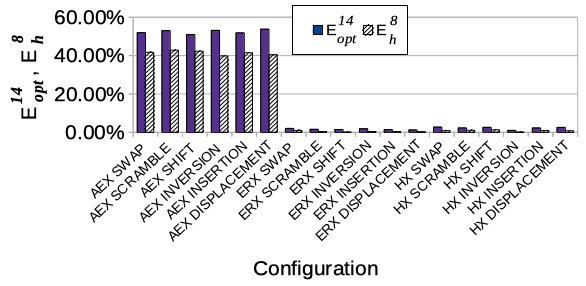
\includegraphics[width=\textwidth]{9_2_Adj_less_100}
		\caption{AEX, ERX, and HX}
		\label{fig:9_2_Adj_less_100}
	\end{subfigure}
	\hfill
	\begin{subfigure}[t]{0.45\textwidth}
		\centering
		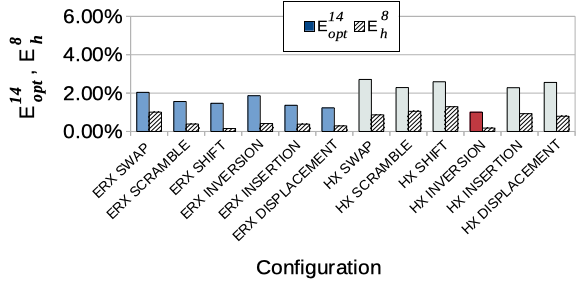
\includegraphics[width=\textwidth]{9_2_ERX_HX_less_100}
		\caption{ERX and HX}
		\label{fig:9_2_ERX_HX_less_100}
	\end{subfigure}	
	\caption{Relative error for instances with less than 100 cities.}
	\label{fig:9_2_less_100}
\end{figure}

In the group of TSP instances with less than 100 cities (see Figure \ref{fig:9_2_Adj_less_100}), the AEX has shown much worse results than the ERX and the HX. Its bad performance in our experiments confirms the results reported in the literature (see \cite{grefenstette1985genetic}) and can be easily explained by the fact that the AEX simply alternately takes the edges from the parents.\par 
 If we compare the ERX and the HX in detail (see Figure \ref{fig:9_2_ERX_HX_less_100}), we can see that the HX combined with the inversion mutation gives the best results. Please note that for small instances of this group which have less than 30 cities, our genetic algorithm has found the optimal value in many configurations.\par 

It is not surprising that for this group of instances with less than 100 cities, the HX performed much better than the AEX: The HX works with the information about the distances between the cities which is extremely relevant for the TSP. However, the fact that the HX did not perform considerably better than the ERX is rather surprising. As it was explained in Section  \ref{subsec:adjacency_crossovers}, the ERX does not uses the domain information like the HX does. It just iteratively takes an edge from the parents which has the smallest number of neighbors. Probably, this was already enough to come to such good results for small instances. Moreover, as it was mentioned in Section \ref{subsec:adjacency_crossovers}, the HX tends to repeat the parents if the number of genes is small. Perhaps that is the reason why the HX does not outperform the ERX on the small instances. \par 

As the winner combination for this group of instances, we choose the HX with inversion as it has shown the best results with respect to $E_{opt}$. Please note that the ERX with shift mutation has shown slightly better results concerning $E_{h}$. However, the number of instances which were used for computing $E_{h}$ is considerably smaller than the number of instances which were used for computing $E_{opt}$. We thus assume that the results with respect to $E_{opt}$ are more stable.\par 

If we take a look at Table \ref{Tab:tab_9_2_adj_less_100}, there is no clear tendency concerning a certain mutation type. One can say that the shift,  inversion and displacement mutation operators perform slightly better than the others. However, the crossover operators show here much stronger influence on the results. It can be easily explained by the fact that these mutation operators were not explicitly developed for the adjacency representation. They do not preserve edges from the parents and make rather random changes. One can therefore make an assumption that applying these mutation operators here can even make the results worse. However, we have conducted a small experiment where we did not use the mutation with the adjacency operators at all: The results without applying mutation were worse than when the mutation takes place. Therefore, we can conclude that mutation is a very important component of genetic algorithms even if one uses the mutation operators which are not perfectly suited for the chosen crossover operators. \par 

 \begin{table}[htp] \centering
	\centering
	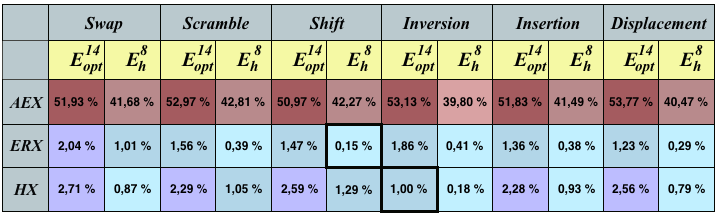
\includegraphics[width=0.8\textwidth]{tab_9_2_adj_less_100}
	\caption{Results for 22 instances with less than 100 cities for AEX, ERX, HX operators and 6 mutation operators.}
	\label{Tab:tab_9_2_adj_less_100}
\end{table}


\begin{figure}[htp] \centering
	\begin{subfigure}[t]{0.45\textwidth}
		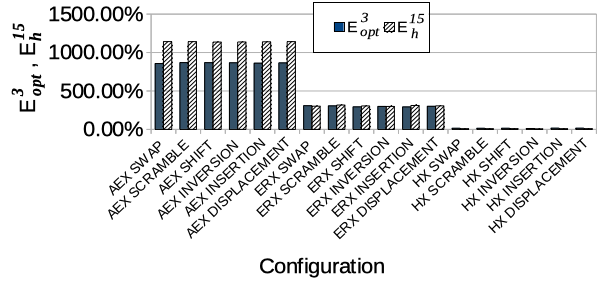
\includegraphics[width=\textwidth]{9_2_Adj_200_500}
		\caption{AEX, ERX, and HX}
		\label{fig:9_2_Adj_200_500}
	\end{subfigure}
	\hfill
	\begin{subfigure}[t]{0.45\textwidth}
		\centering
		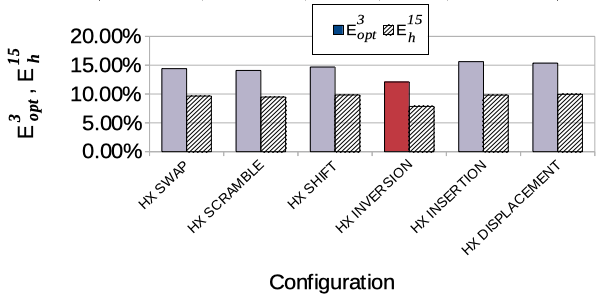
\includegraphics[width=\textwidth]{9_2_HX_200_to_500}
		\caption{HX}
		\label{fig:9_2_HX_200_to_500}
	\end{subfigure}	
	\caption{Relative error for instances with 200 to 500 cities.}
	\label{fig:9_2_200_to_500}
\end{figure}

Now let us take a look at the results which were obtained for the TSP instances with 200 to 500 cities  (see Figure \ref{fig:9_2_Adj_200_500}). One can see here a significant difference among the three crossover operators: The AEX performs worst again, the ERX shows better results, but the definite winner is the HX again. The middle results of the ERX here correspond more to our expectations than the results for smaller instances. The outperformance of the HX is not surprising as well because this operator uses the information which is very relevant for the TSP.  Therefore, it is better applicable to the TSP problem. If we take a look at this crossover type more in detail, than we can see that the combination with the inversion mutation is slightly better than the others (see Figure \ref{fig:9_2_HX_200_to_500}).\par  

 \begin{table}[htp] \centering
	\centering
	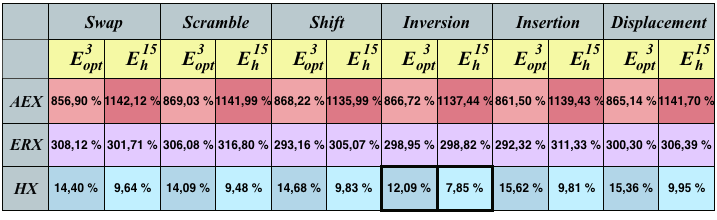
\includegraphics[width=0.8\textwidth]{tab_9_2_adj_200_to_500}
	\caption{Results for 18 instances with 200 to 500 cities for AEX, ERX, HX operators and 6 mutation operators.}
	\label{Tab:tab_9_2_adj_200_to_500}
\end{table}

If we take a look at Table \ref{Tab:tab_9_2_adj_200_to_500}, we again observe that the mutation operator does not seem to influence the results. No mutation type can be found which has consistently better results than the other. Here, the influence of crossover types is significantly stronger.\par 

Summarizing the results of this part of our experiments, the HX in combination with the inversion mutation has performed best for both groups of instances and is considered as the winner for the adjacency representation crossovers.\par

\subsection{Ordinal Representation with OPX}
\label{subsec:experiments_ordinal}

\subsubsection{Methods}

For the ordinal representation, we consider the classical one-point crossover (OPX) (see Section \ref{subsec:opx}). It was claimed \cite{potvin1996genetic} that this representation type is only of historic interest because it has shown very bad results. The purpose of this experiment is to validate this claim on our dataset. Moreover, we will combine this crossover type with 6 different mutation types, namely swap, shift, scramble, inversion, insertion, and displacement. As a result, we get 6 configurations in total.\par  

\subsubsection{Results and Discussion}

In the group of TSP instances with less than 100 cities, the OPX has shown the best results in combination with the inversion mutation and the worst ones with the scramble mutation (see Figure \ref{fig:9_3_opx_less_100}).

\begin{figure}[htp] \centering
	\centering
	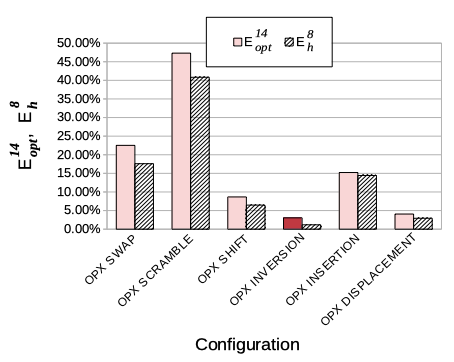
\includegraphics[width=0.6\textwidth]{9_3_opx_less_100}
	\caption{Results for 22 instances with less than 100 cities for the OPX and 6 mutation operators.}
	\label{fig:9_3_opx_less_100}
\end{figure}

\begin{figure}[htp] \centering
	\centering
	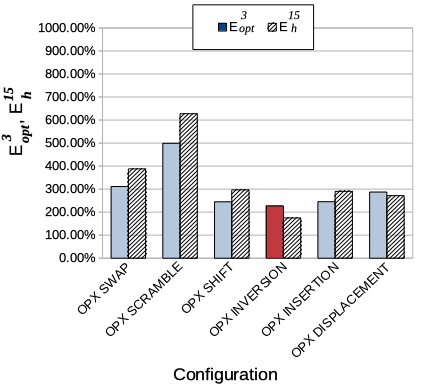
\includegraphics[width=0.6\textwidth]{9_3_opx_200_to_500}
	\caption{Results for 18 instances with 200 to 500 cities for the OPX and 6 mutation operators.}
	\label{fig:9_3_opx_200_to_500}
\end{figure}

In the group with larger instances with 200 to 500 cities, the OPX has also shown the best results combined with the inversion mutation and the worst ones with the scramble mutation (see Figure \ref{fig:9_3_opx_200_to_500}).\par 

Whether this crossover type can compete with the crossover operators of other representation types, will be validated in the next section, where we are going to compare the results among the representation types.\par 

\subsection{Best and worst mutation operators}
\label{subsec:experiments_mutation}

Summarizing the results of the previous sections, we can definitely state that the inversion mutation has always shown the best results for all crossover operators while the scramble mutation has performed poorly. A great importance of inversion was also described by \citeauthor{potvin1996genetic} \cite{potvin1996genetic}. One can explain it by the fact that the inversion mutation changes only two edges preserving the other ones (see Section \ref{sec:mutation}). It changes only the edges which stand at the start and the end of the interval where the inversion happens. Strictly speaking, the other edges can be changed as well but these changes may affect only the direction. However, a change in direction does not influence the length of the tour in symmetric TSP instances, and it does not therefore affect the fitness value. \par 

\begin{figure}[htp] \centering
	\begin{subfigure}[t]{0.45\textwidth}
		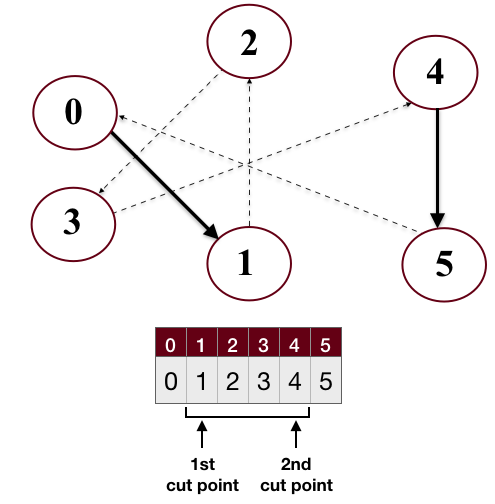
\includegraphics[width=\textwidth]{9_initial_graph}
		\caption{Graph for the chromosome encoding the tour 012345.}
		\label{fig:9_initial_graph_1}
	\end{subfigure}
	\hfill
	\begin{subfigure}[t]{0.45\textwidth}
		\centering
		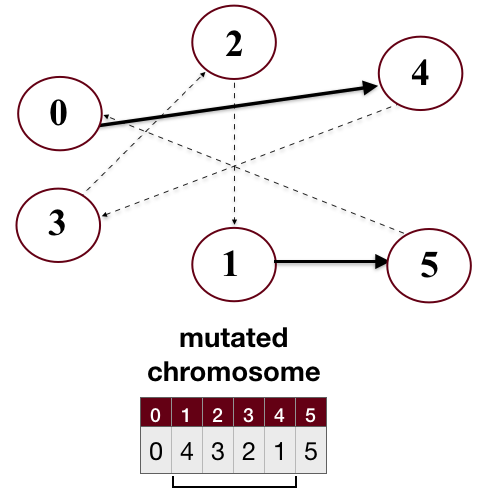
\includegraphics[width=\textwidth]{9_inversion_done}
		\caption{Applying the inversion mutation with the cut points 1 and 4}
		\label{fig:9_inversion_done}
	\end{subfigure}	
	\caption{Changes in the graph while applying the inversion mutation with the cut points 1 and 4.}
	\label{fig:9_inversion_changes_graph}
\end{figure}

 For instance, consider the chromosome which encodes the tour 012345 in path representation. Let us assume that the cut points are 1 and 4 between which the inversion will happen (see Figure \ref{fig:9_initial_graph_1}). This means that the edge (0,1) stands at the beginning of the interval and the edge (4, 5) stands at the end of it. Applying the inversion here removes these two edges and produces two new edges (0, 4) and (1, 5) (see Figure \ref{fig:9_inversion_done}). \par 

\vspace{2cm}

On the other side, applying a scramble mutation to the same chromosome with the same cut points can result into destroying almost all edges (see Figure \ref{fig:9_scramble_changes_graph}). These changes can therefore completely destroy the results of the crossover operators.\par 


\begin{figure}[htp] \centering
	\begin{subfigure}[t]{0.45\textwidth}
		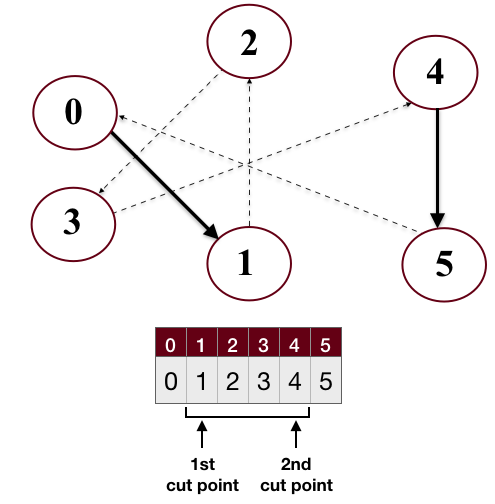
\includegraphics[width=\textwidth]{9_initial_graph}
		\caption{Graph for the chromosome encoding the tour 012345.}
		\label{fig:9_initial_graph_2}
	\end{subfigure}
	\hfill
	\begin{subfigure}[t]{0.45\textwidth}
		\centering
		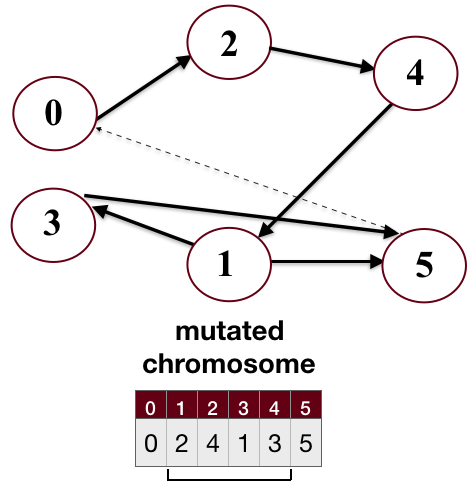
\includegraphics[width=\textwidth]{9_scramble}
		\caption{Applying the scramble mutation with the cut points 1 and 4.}
		\label{fig:9_scramble}
	\end{subfigure}	
	\caption{Changes in the graph while applying the scramble mutation with the cut points 1 and 4.}
	\label{fig:9_scramble_changes_graph}
\end{figure}




 